\documentclass[12pt]{exam}
\usepackage{amsthm}
\usepackage{bm}
\usepackage{libertine}
\usepackage[utf8]{inputenc}
\usepackage[margin=0.5in]{geometry}
\usepackage{amsmath,amssymb}
\usepackage{multicol}
\usepackage[shortlabels]{enumitem}
\usepackage{siunitx}
\usepackage{physics}
\usepackage{booktabs}
\usepackage{graphicx}
\usepackage{pgfplots}
\usepackage{listings}
\usepackage{tikz}
\usepackage{tikz-3dplot}

\bmdefine{\ii}{i}                       %% cuaternion i
\bmdefine{\jj}{j}                       %% cuaternion j
\bmdefine{\kk}{k}                       %% cuaternion k
\newcommand{\te}{\theta}                %% short for  \theta
\newcommand{\cC}{\mathcal{C}}

\newcommand{\word}[1]{\quad\text{#1}\quad} %% texto intercalado


\pgfplotsset{width=10cm,compat=1.9}
\usepgfplotslibrary{external}
\tikzexternalize

\newcommand{\class}{Math 261-001} % This is the name of the course 
\newcommand{\examnum}{Quiz 8} % This is the name of the assignment
\newcommand{\examdate}{October 31} % This is the due date





\begin{document}
\pagestyle{plain}
\thispagestyle{empty}

\noindent
\textbf{\class}\\
\textbf{\examnum}, \textbf{\examdate} \\

% Name \hfill CSU ID \# \hspace{2.25in}

%\vspace{10 pt}

\setlength{\tabcolsep}{3.5cm} % Default value: 6pt
\renewcommand{\arraystretch}{1.5}
\setlength\extrarowheight{1cm}
\begin{tabular}{ |c|c| } 
 \hline
 Name   & CSU ID \#  \\ 
 \hline
\end{tabular}
% ---
\vspace{10pt}
\iffalse

    \foreach \s in {1,...,5}{
          \choice $P_\s$ has no power 
     }%;
\fi

Be sure to read each question carefully. You must choose and answer \textbf{exactly two} of the three problems.  
If you attempt more than two, only the first two will be graded.  
Write your final answers in the boxes provided. Each problem is worth the same number of points.  
\textbf{Each problem is accompanied by a figure to help you visualize the region in question.}  

\begin{enumerate} 

\item While on the supermarket you eye the 60 egg carton (\textit{great deal btw}) formed by stacking two cartons on top of each other. Lost in thought, you idealize the carton having the shape
$$ z=\frac12\cos(4x)+\frac12\sin(4y),\word{with} -2\leq x,y\leq 2.$$
You ponder thoroughly and realize this surface is written as a function of $x$ and $y$. Given this information, write an expression (only setup, no calculation) for the area of the surface of one such carton. 
\vfill
\begin{flushleft}
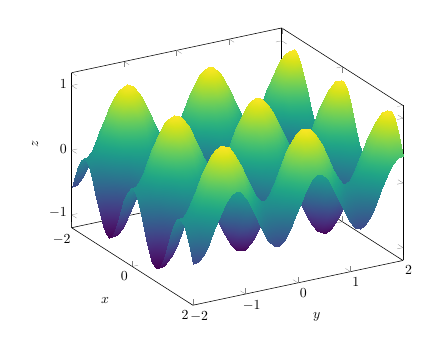
\begin{tikzpicture}[scale=0.5]
\begin{axis}[
    view={60}{30},
    domain=-2:2,
    domain y=-2:2,
    samples=40,
    samples y=40,
    xlabel={$x$},
    ylabel={$y$},
    zlabel={$z$},
    colormap/viridis,
    mesh/ordering=y varies,
]
\addplot3[
    surf,
    shader=interp,
]
{0.5*cos(deg(4*x)) + 0.5*sin(deg(4*y))};
\end{axis}
\end{tikzpicture}
\end{flushleft}
\begin{flushright}
\framebox(320,50){}
\end{flushright}

\item You bought one of those pieces of cheese ball with the red peel. Before throwing away the peel you decide it's time to test yourself and see whether you can parametrize it. Assume the cheese ball has radius $3$ and the piece you got is bounded below by the $xy$ plane and on the side by the $xz$ plane. Given this, parametrize the described peel.
\vfill
\begin{flushleft}
  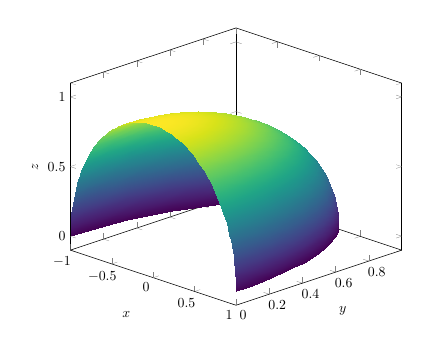
\begin{tikzpicture}[scale=0.5]
\begin{axis}[
    view={45}{25},
    domain=0:pi,
    y domain=0:pi/2,
    samples=40,
    samples y=40,
    xlabel={$x$},
    ylabel={$y$},
    zlabel={$z$},
    colormap/viridis,
    z buffer=sort,
]
\addplot3[
    surf,
    shader=interp,
]
({cos(deg(x))*cos(deg(y))},
 {sin(deg(x))*cos(deg(y))},
 {sin(deg(y))});
\end{axis}
\end{tikzpicture}
\end{flushleft}
\begin{flushright}
\framebox(320,50){}
\end{flushright}

\newpage
\item Recall that integrating a vector field $F$ through a surface can be done by computing $\iint_{S} F(r)\cdot\vec{n}\dd A$ where $\vec{n}$ is the normal vector to the surface $S$ parametrized by $r$.\par
Given the surface $x+y+z=1$ and the vector field $F=(0,0,z)$, compute the integral $\iint_{S} F(r)\cdot\vec{n}\dd A$. (Your answer should be a number, not an integral.)
\begin{flushleft}
 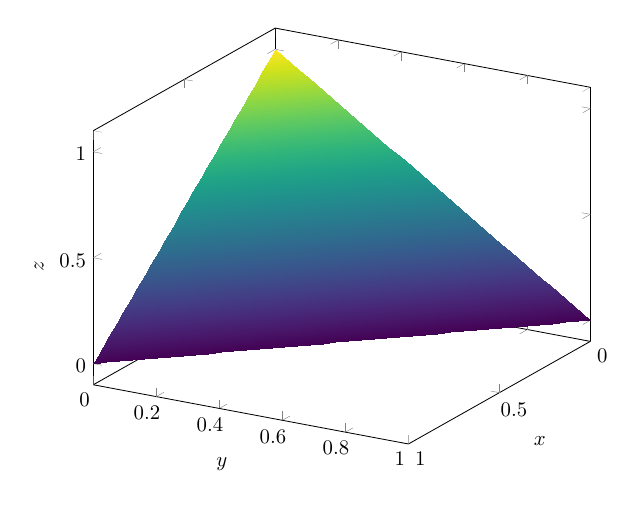
\begin{tikzpicture}[scale=0.75]
\begin{axis}[
    view={120}{25},
    domain=0:1,
    y domain=0:1,
    samples=40,
    samples y=40,
    xlabel={$x$},
    ylabel={$y$},
    zlabel={$z$},
    z buffer=sort,
    colormap/viridis,
]
\addplot3[
    surf,
    shader=interp,
]
({x*y}, {x*(1 - y)}, {1 - x});
\end{axis}
\end{tikzpicture}
\end{flushleft}
\vfill
\begin{flushright}
\framebox(350,50){}
\end{flushright}

\end{enumerate}


\end{document}

